\section{Introduction}
\label{sec:intro}

%SSO的特点
%SSO的现状
Single sign-on (SSO) systems, such as OAuth~\cite{rfc6749}, OpenID Connect~\cite{OpenIDConnect} and SAML~\cite{SAML}, have been widely adopted nowadays as a convenient web authentication mechanism. SSO delegates user authentication from websites, so-called relying parties (RPs), to a third party, so-called identity providers (IdPs), so that users can access different services at cooperating sites via a single authentication attempt. Using SSO, a user no longer needs to maintain multiple credentials for different RPs, instead, she maintains only the credential for the IdP, who in turn will generate corresponding \emph{identity proofs} for those RPs. Moreover, SSO shifts the burden of user authentication from RPs to IdPs and reduces security risks and costs at RPs. As a result, SSO has been widely integrated with modern web systems.
%实际数据
%The survey on the top 100 websites from SimilarWeb~\cite{similarweb} demonstrates that only 25 websites (excluding the ones not for browser accessing) do not integrate the SSO service.
Our study shows that 80\% of the Alexa top-100 websites~\cite{Alexa} support SSO services and study on the Alexa top 1 million websites has found that 6.30\% of websites support  SSO~\cite{GhasemisharifRC18}.
Meanwhile, many email and social networking providers such as Google, Facebook, Twitter, etc. have been actively serving as social identity providers to support social login.


%SSO系统的安全问题,需要保护identity proof的完整性,机密性,绑定性
%完整性:使用公开的为受保护的信息作为identity proof
%机密性:保证由IdP发送给对应的RP,并且传输过程中通道、user agent都是受到保护的
%绑定性:identity proof一定要与对应的RP实现绑定
A fundamental requirement of SSO systems is secure authentication~\cite{SPRESSO}, which should ensure that it is impossible (1) for an adversary to log in to an honest RP as an honest user (i.e., impersonation); and (2) for an honest user to log in to an honest RP as someone else such as an adversary (i.e., identity injection).
Extensive study have been performed on existing SSO systems exposing various vulnerabilities~\cite{ChenPCTKT14, FettKS16,WangCW12,ZhouE14,WangZLG16,YangLLZH16,SomorovskyMSKJ12,MohsenS16}. It is commonly recognized that SSO security highly depends on secure generation and transmission of identity proofs: (1) the identity proof should be generated in a way that it can never be forged or tampered. For example, when Google used user's attributes with a signature as the identity proof~\cite{WangCW12}, {\color{red}the adversary is able to bypass the verification of part of attributes in the identity proof. The root cause is that RP relies on the IdP signed user's attributes to identify the user, however, when the adversary acts as the user, it is able to modify the request and repose between RP and IdP transmitted by user, which allows the adversary add any honest user's attributes in the IdP's response and RP would accept all of them without verifying the signature. Finally the adversary is able to log in to the RP as the honest user}.
(2) The identity proof should be generated in a way that it is bound to the requesting RP. For example, if an identity proof is generated with nonbinding data such as access tokens in OAuth 2.0, an adversary such as a malicious RP is able to log in to an honest RP as the honest user~\cite{ChenPCTKT14, WangZLG16}.
%the parts of IdP developer choose the data (e.g., access token in OAuth 2.0) unbound with specific RP as the identity proof, which results in that the malicious RP is able to collect user's identity proof and use it to log in to other RPs.
(3) The identity proof should only be obtained by the requesting RP. For example, in some mobile SSO implementations using WebView~\cite{MohsenS16}, as the url check is not supported which the malicious RP app invokes the IdP's web site in its Webview, the adversary is able to steal the identify proof of an honest user when the app cheats her to consider it as another honest RP.

%第二段:
%SSO 引入新的隐私问题
%IdP知道用户登录哪个RP
%RP之间可以合谋知道同一个用户登录哪些RP
The wide adoption of SSO also raises new privacy concerns regarding online user tracking and profiling~\cite{maler2008venn,NIST2017draft}. In a typical SSO authentication session, for example the OpenID Connect (OIDC) authentication flow as shown in Fig.~\ref{fig:OpenID}, when a user attempts to log in to an RP, the authentication request is redirected from the RP to the IdP, which generates an identify proof containing information about the user (e.g., user identifier and other authorized user attributes) and the requesting RP (e.g., RP identifier, URL, etc.). If a common user identifier is issued by the IdP for a same user across different RPs or a user's identifiers can be derived from each other, which is the case even in several widely deployed SSO systems~\cite{BrowserID,SPRESSO}, collusive RPs could not only track her online traces but also correlate her attributes across the sites~\cite{maler2008venn}. We refer to this as {\em RP-based identity linkage}. Moreover, when a user leverages the identity issued by one IdP across multiple RPs, the IdP acquires a central role in web authentication, which enables it to collect information about the user's logins at different sites~\cite{maler2008venn}. Since the information of the RP is necessary in the construction of identity proof to make sure it is bound with specific RP~\cite{ChenPCTKT14, WangZLG16}, any interested IdP can easily discover all the RPs accessed by a user and reconstruct her access traces by the unique user identifier. We refer to this as {\em IdP-based access tracing}. Both RP-based identity linkage and IdP-based access tracing could lead to more severe privacy violations.

%Instead of maintaining the user's information (including identifier) independently in those systems not integrating the SSO service,  the IdP maintains the user's attributes  and identity proof in SSO systems, which allows the IdP or the collusive RPs to infer the access trace of a specified user~\cite{NIST}. In details, the privacy leakage risks include:
%It has already been discussed in the NIST Special Publication 800-63C~\cite{NIST}. In details, the privacy leakage risks include:


%第三段:
%google and facebook的负面新闻
%1. service provider(如DNS)知道你访问了,可以带来很多问题。但是还是不同的,DNS里profile需要评估的是two behavior vectors的similarities,而IdP中都不需要,因为IdP能够区分two behavior vectors 是否来自相同节点。

Meanwhile, large IdPs, especially social IdPs like Google and Facebook, are known to be interested in collecting users' online behavioral information for various purposes (e.g., Screenwise Meter~\cite{googlenews}, Onavo~\cite{Onavo}). By simply serving the IdP role, these companies can easily collect a large amount of continuous data to reconstruct users' online traces. %Unlike other privacy risks, such as user session re-identification that requires to compute the similarity between users' DNS queries~\cite{DNS},
Moreover, many service providers are also hosting a variety of web services, which make them easy to link the same user's multiple logins in each RP as the unique user identifier is contained in the identity proof. Through internal integration, they could obtain rich information from SSO data to profile their clients.

%As suggested in NIST SP800-63C~\cite{NIST2017draft}, to protect users' privacy, in SSO systems, 1) the user should be able to control the range of the attributes exposed to the RP, 2) multiple RPs should fail to link the user through collusion, 3) IdP should fail to obtain the trace of RPs accessed by a user. The first property is satisfied in most SSO systems. For example, in OAuth and OIDC, IdP exhibits the  attributes requested by the RP and sends the attributes to the RP only when the user has provided a clear consent, which may also minimize the exposed attributes as the user may disagree to provide partial attributes.

%However, exposing accessed RP to IdP is required for security consideration in existing SSO systems~\cite{ChenPCTKT14}. Firstly, the identity proof should only be sent to the correct RP, which prevents the adversary from performing the impersonation attack with the leaked identity proof. Secondly, the identity proof should be bound with a specific RP and user, which ensures the identity proof is only valid in the certain RP, and avoids the misuse of identity proof, for example, the adversary fails to  use the identity proof for a corrupted RP to  access another RP on behalf of the victim user.

%~\cite{SAMLIdentifier,OpenIDConnect,persona,SPRESSO} are proposed to protect the user's privacy in SSO systems, either achieving the identity unlinkage~\cite{SAMLIdentifier,OpenIDConnect}, or preventing the IdP from tracing the users~\cite{persona,SPRESSO}.

While the privacy problems in SSO have been widely recognized~\cite{maler2008venn,NIST2017draft}, only a few solutions have been proposed to protect user privacy~\cite{persona,SPRESSO}. Among them, Pairwise Pseudonymous Identifier (PPID)~\cite{OpenIDConnect, SAMLIdentifier} is a most straightforward and commonly accepted solution to defend against RP-based identity linkage, which requires the IdP to create different user identifiers for the user when she logs in to different RPs. In this way, even multiple malicious RPs collude with each other across the system, they cannot link the  pairwise pseudonymous identifiers of the user and track which RPs she has visited. As a recommended practice by NIST~\cite{NIST2017draft}, PPID has been specified in many widely adopted SSO standards including OIDC~\cite{OpenIDConnect} and SAML~\cite{SAMLIdentifier}.

However, PPID-based approaches cannot prevent the IdPs from tracking at which RPs users log in, since pseudonymous identifiers are generated by IdP which only hide users' identity from the RPs. To authenticate a user, the IdP has to know her identity. To the best of our knowledge, there are only two approaches (i.e., BrowserID~\cite{BrowserID} and SPRESSO~\cite{SPRESSO}) being proposed so far to prevent IdP-based access tracing. Both adopt the idea of hiding RPs' identities from the IdP during the construction and transmission of identity proofs. In particular, the identity proof in BrowserID (and its prototype system known as Mozilla Persona~\cite{persona} and Firefox Accounts~\cite{FirefoxAccount}) is combined with two parts, the binding of the public key generated by the user with her email (as the user identifier) signed by IdP as the user certificate (UC) and the origin of the RP signed by user's private key as the identity assertion (IA). The core idea of BrowserID is that the IdP-generating part of identity proof does not contains any RP's identity and the work of binding identity proof with RP is shift to the user. 
% uses email address as user identifier, and lets the IdP bind the public key generated by the user with her email. The identity proof , the signed with the corresponding private key of the user and transmitted to the RP via the user. 
With the user as the proxy, the IdP does not know RPs' identities throughout the authentication process. 
In SPRESSO, the RP generates a dynamic pseudonymous identifier by encrypting its domain and a nonce, and passes it to the IdP through the user to create the identity proof, which is returned to the RP through a trusted third party, called forwarder, chosen by the RP itself. While forward transmitting the identity proof, it decrypts the encrypted RP domain to make sure the identity proof only sent to the requesting RP, however, the identity proof is encrypted by another RP generated symmetric key before transmitting to avoid the forward knowing the user's identity from identity proof, which will result in the forward tracing the user. As it designed in SPRESSO, the user email is adopted as the user identifier for identity proof generating. 

%In BrowserID, the identity proof is signed with the private key generated by user, and transmitted to the RP through the user directly,  while the corresponding  public key is bound with users' email by IdP who need not obtain the information of accessed RP. In SPRESSO, RP encrypts its domain and a nonce as the identifier, so that the real identity of RP is never exposed to IdP, while the identity proof is transmitted to the RP through a trusted entity (named FWD) who doesn't know the user's identity.

%To prevent IdP tracing the RPs accessed by the user, two SSO systems (BrowserID~\cite{persona} and SPRESSO~\cite{SPRESSO}) are proposed to hide the user's accessed RPs from IdP who fails to obtain the information of accessed RP. In BrowserID, the identity proof is signed with the private key generated by user while the corresponding  public key is bound with users' email by IdP who need not obtain the information of accessed RP. In SPRESSO, RP uses the encrypted RP domain and a nonce as the identifier, so that the real identity of RP is never exposed to IdP.


%although the designs of SSO system make the effort to protect users' privacy,
%However, there is no existing SSO system which prevents both the access tracing and identity linkage. The implementations of OIDC and SAML prevent the identity linkage, but allow the IdP to obtain the identifiers of accessed RPs, while BrowserID and SPRESSO are designed to avoid the IdP to obtain the access tracing, but the colluded RPs may still link the user as the unique email address is used as the identifier in all RPs.
%However, there is no existing SSO system protecting users' privacy comprehensively. Currently proposed designs for privacy protection are only available in dealing with one privacy leaking problem, none of these systems are able to deal with the both privacy issues at the same time. Therefore, it means that the adversary always have at least one way to track users.


%用户和每一个RP分别在IdP处有长期不变的ID,分别称为ID_U和ID_RP;IdP为用户签发的identity proof中存在着连接ID_U和ID_RP的ID,称为ID_U^Proof;用户在每一个RP处都有长期不变的Account。
%在每一次identity proof产生的过程中(也就是每一次log in rp),IdP会产生绑定了ID_U和ID_RP的identity proof
%原始的SSO方案中,会同时暴露ID_U和ID_RP
%为了保护用户隐私,应该保证ID_U与ID_U^RP不同,并且ID_U^RP在不同的RP不同,同时应该使用变换后的随机ID_RP代表RP身份
%在PPID方案中,ID_U与ID_U^RP不同,防止了RP-based linkage,但是向IdP暴露了ID_RP
%在SPRESSO中,使用了加密的ID_RP代表RP身份,但是ID_U与ID_U^RP相同
%in this paper, we propose xxxx。
%具体的,在我们的方案,,Account和ID_U不同;同时,在每一次identity proof 产生的过程之中,RP都会在IdP处动态地注册匿名ID,称为PID_RP;同时,IdP会根据PID_RP和IDU产生PID-U,并将PID_RP和PID-U绑定在identity proof中;当RP验证了identity proof之后,会利用PID_RP生成过程中存在的trapdoor得到不变的account。
%我们的方案满足(1)(2)(3)
Unfortunately, %none of the existing approaches provides sufficient and comprehensive protection for user security and privacy in SSO. For example, \cite{BrowserID} reported that BrowserID suffered from a severe privacy attack in which malicious IdPs could check users' login status at any RP. We also find that the security of SPRESSO highly relies on the third-party forwarder and therefore it is vulnerable to the impersonation attacks once the chosen forwarder is compromised. Moreover,
none of the existing SSO systems could address both RP-based identity linkage and IdP-based access tracing privacy problems at the same time.
The user's identity is represented by several forms in different environments. In detail, the IdP and RP store the unique user identifier (denoted as $ID_U$ in IdP and $Account$ in RP) for each users solely, which are linked by the identity proof containing the junctional user identifier (denoted as $ID_U^{Proof}$) issued by IdP. Moreover, there is also the unique RP identifier (denoted as $ID_{RP}$) stored in IdP. In each authentication, the identity proof issued by IdP should contain the $ID_{RP}$ (making sure the identity proof is issued for specific RP) and $ID_U^{Proof}$ (for RP to identify the user). In some traditional SSO systems~\cite{rfc6749}, the $ID_U$ and $ID_U^{Proof}$ are the same one, which results in the RP-based identity linkage, and the $ID_{RP}$ is always exposed to IdP, which results in the IdP-based access tracing. However, to avoid the privacy problems in SSO systems, the $ID_U^{Proof}$ should not be the same as the RP (or the $ID_U^{Proof}$ should not be the same in different RPs) and the $ID_{RP}$ should not be exposed to the IdP (using a transformed $ID_{RP}$ representing the RP) in each authentication. The widely adopted SSO standards, such as OIDC and SAML, use $PPID$ as the $ID_U^{Proof}$ transformed from $ID_U$ which is constant in one RP but different in RPs, but expose the $ID_{RP}$ straightforward to the IdP. Otherwise, the SPRESSO adopts the encrypted $ID_{RP}$ (denoted as $enc(ID_{RP})$) and only the $enc(ID_{RP})$ is exposed to the IdP, however, the $ID_U^{Proof}$ is the same one as the $ID_U$ in SPRESSO. As for the BrowserID, the identity proof is generated by the cooperation between IdP and user so that it could avoid exposing $ID_{RP}$ to IdP, but uses same identifier for $ID_U$ and $ID_U^{Proof}$. The worse thing is there is not a simple way to combine the existing schemes together to protect user's privacy comprehensively (the details are described in Section~\ref{sec:challenge}).

In this paper, we propose UPRESSO, an Unlinkable Privacy-REspecting Single Sign-On system, as a comprehensive solution to tackle the privacy problems in SSO. We propose novel identifier generation schemes to dynamically generate  privacy-preserving $ID_U^{Proof}$ and transformed $ID_{RP}$, denoted as $PID_U$ and $PID_{RP}$, to construct identity proofs for SSO. In our scheme, for each login, RP anonymously registers a random $ID_{RP}$ (denoted as $PID_{RP}$) with IdP, and exposes the $PID_{RP}$ for authentication. IdP generates the $PID_U$ with $PID_{RP}$ and $ID_U$ and issues the identity proof containing $PID_{RP}$ and $PID_U$. Finally, after RP validates the identity proof, it utilizes the trapdoor obtained when generating the $PID_{RP}$ to derive the $Account$ from $PID_U$. However the scheme must satisfy three properties: (1) when a same or differnt user(s) log in to a same RP, random $PID_{RP}$s are generated in different logins so that a curious IdP cannot infer the real identity of the RP or link multiple logins at that RP; (2) when a same user logs in to a same or different RPs, random $PID_U$s are generated so that collusive RPs cannot link the logins of that user; (3) when a same user logs in to a same RP, the RP can derive a unique user identifier from different PUIDs with a trapdoor so that it can provide a continuous service to the user during different logins.

\begin{figure}
  \centering
  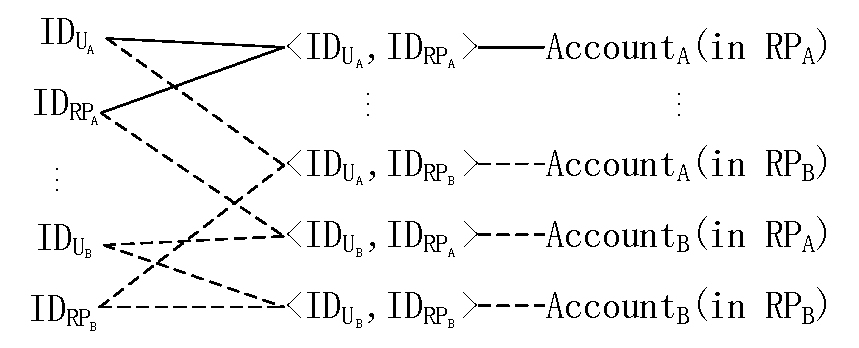
\includegraphics[width=\linewidth]{fig/link1.pdf}
  \caption{Traditional SSO.}
  \label{fig:TraditionalSSO}
\end{figure}
\begin{figure}
  \centering
  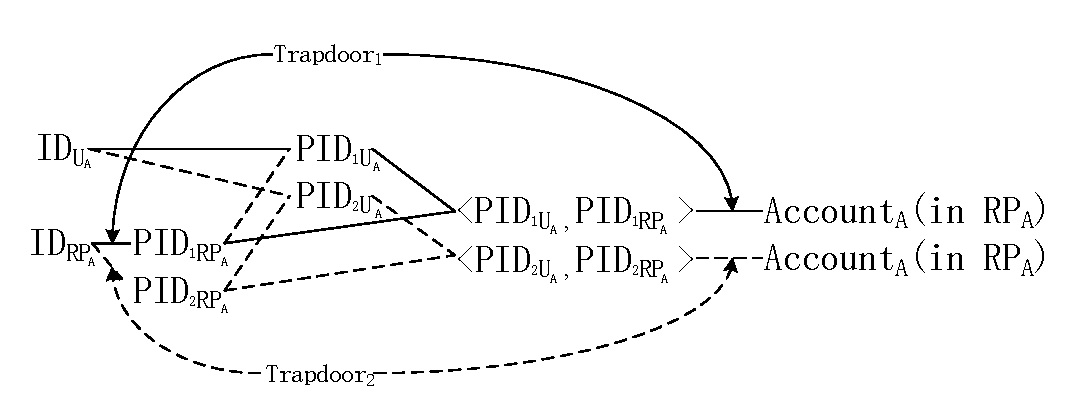
\includegraphics[width=\linewidth]{fig/link2.pdf}
  \caption{Our scheme.}
  \label{fig:Ourscheme}
\end{figure}


%In BrowserID and SPRESSO, collusive RPs could link a user's multiple logins from the common user identifier.
%In this paper, we present UPRESSO, an Unlinkable Privacy-REspecting Single Sign-On system,
%UPRESSO, privacy-\(RE\)specting single sign-On system a\(C\)hieving un\(L\)inkable \(USE\)rs' traces
%as a comprehensive solution to tackle the privacy problems in SSO. We propose novel identifier generation schemes to dynamically generate  privacy-preserving user and RP identifiers, denoted as $PUID$ and $PRPID$, to construct identity proofs for SSO, which satisfy three properties: (1) when a same or differnt user(s) log in to a same RP, random $PRPID$s are generated in different logins so that a curious IdP cannot infer the real identity of the RP or link multiple logins at that RP; (2) when a same user logs in to a same or different RPs, random $PUID$s are generated so that
%neither a curious IdP nor
%collusive RPs cannot link the logins of that user; (3) when a same user logs in to a same RP, the RP can derive a unique user identifier from different PUIDs with a trapdoor so that it can provide a continuous service to the user during different logins.

%from both the IdP and RPs, named {UPRESSO}. To achieve this, we rely on the user to achieve the trusted transmit and correctness check of identity proof (same as in BrowserID~\cite{persona}), and propose two algorithms to achieve:

%{\color{blue} To achieve this, we propose the novel method to enable the IdP to generates the pairwise user identifier with the RP's one-time identity, which never exposes the RP's real identity. The method is consisted of RP's identifier generation and PPID generation, where two algorithms are proposed to achieve:}

\begin{comment}

\begin{itemize}
\item RP's identifier generation and transformation, which makes the RP's identifier in multiple authentications  different, and IdP fails to infer RP's information or link it in different authentications. Moreover, neither RP nor the user may control the generated identifier, which avoids the misuse of the identity proof. The detailed analysis is provided in Section~\ref{sec:analysis}.
\item PPID generation, which makes the PPIDs for one user in one RP indistinguishable from others (e.g., different users in different RPs), while only the RP (and the user) has the trapdoor to derive the unique identifier from different PPIDs for one user in one RP.
\end{itemize}

\end{comment}

%{\color{blue} Besides, we also propose a way to shift the responsibilities of trusted transmit and correctness check of identity proof from IdP to user. }


%In this paper, we propose the first scheme which deals with all the privacy issues introduced by SSO comprehensively. UPRESSO enables the RP to hide its identity from IdP for users authentication, as well as IdP is able to provide distinct user identifiers for each RP. To achieve the above goals, we  proposed the scheme for RP and user identifier generating, which allows that, 1) RP has the ability to offer the changing RP identifiers to IdP in each authentication, from which the real RP identity is not possible to be derived without the trapdoor; 2) IdP is able to generate unique user identifier (\verb+user_idp_id+) bound with specific RP identifier, from which the user identifier in RP(\verb+user_rp_id+)is to be derived with the trapdoor. However, multiple RPs are unable to link the user by \verb+user_rp_id+ or \verb+user_idp_id+.

Unlike previous approaches that require non-trivial re-design of the existing SSO systems, UPRESSO can be implemented over a widely used OIDC system with small modifications with the support of its dynamic registration function~\cite{DynamicRegistration}.

%Reluse only requires the following modification on  OIDC implementations: (1) an additional web service at the IdP for providing a  set of public parameters; (2) the support for generating  the new RP identifier (at the user and RP), PPID (at the IdP) and user's account (at RP). The prototype demonstrates  that UPRESSO is incompatible with existing OIDC implementations.

%Compared with BrowserID and SPRESSO, UPRESSO does not only deal with the privacy issues comprehensively but also be compatible with traditional OIDC system, which is not achieved by neither BrowserID and SPRESSO. BrowserID requires that the user's identity proof should be generated by user's browser, as well as SPRESSO has to introduce new trustful party into the system.
%To deal with the security considerations introduced by hiding RP in OIDC: 1) the identity proof should only be sent to the correct RP; 2) identity proof should not be misused. The following requirements should be fulfilled by UPRESSO:
%\begin{itemize}
%\item A new algorithm is proposed to negotiate the RP's identifier between the user and RP for each login. Therefore, the RP's identifier in multiple authentications are different, and IdP fails to infer RP's information or link it in different authentications. Moreover, neither RP nor the user may control the generated identifier, which avoids the misuse of the identity proof. The detailed analysis is provided in Section~\ref{sec:analysis}.
%302跳转可以不产生referer
%\item A browser extension is introduced to transmit the messages (i.e.,  request and response) related with the authentication, which ensures only the correct RP receives the id token.
%\item A new generation algorithm of PPID is provided, which makes the PPIDs for one user in one RP  indistinguishable  from others (e.g., different users in different RPs), while only the RP (and the user) has the trapdoor to derive the unique identifier from different PPIDs for one user in one RP.
%\end{itemize}
%We implement UPRESSO prototype as follows: the IdP is based on the MITREid Connect, RP is a Java web service based on the SpringMVC framework and a chrome extension for the functions on the user side. %Finally we prove the availability of the UPRESSO and evaluate the delay introduced by UPRESSO.


%In this paper, we propose an extension (named PriOIDC) of existing widely adopted SSO system (i.e., OIDC), which preserves the systematically and thoroughly analyzed security, and achieves the fully privacy. That is, (1) the security design in OIDC is inherited to prevent the impersonation attack and  identity injection attack, (2) the privacy enhance mechanisms (e.g., the clear consent from the user and the PPID) are retained, (3) a new mechanism is introduced to hide the user's accessed RP from IdP. Unlike designing and deploying a new SSO systems, we only need to analyze the compliance of the new function (i.e., hiding the user's accessed RP) and the influence to the security introduced by the new mechanism. And, the deployment of PriOIDC only requires: (1) IdP provides a set of public parameters and generates the PPID with a newly provided algorithm, (2) RP integrates the SSO service with a new version software development kit (SDK) whose interface remains unchanged, (3) the user installs an extension to access RP with full privacy anywhere as no persistent storage is required in the user side.



%Moreover, the basic requirement of SSO systems is the security, which includes two aspects: 1) the attacker should not be able to access the honest RP with the honest users' identity; 2) the identity injection will never succeed, that is, the attacker should not be able to make the honest user access the RP with an incorrect identity. Plenty of works are proposed for the security of SSO systems.
%Firstly, various standards, e.g., OAuth 2.0~\cite{rfc6749}, SAML~\cite{SAML} and OpenID Connect (OIDC)~\cite{OpenIDConnect}, are proposed to formalize the handling at each entity (i.e.,  the user, RP and IdP)  and the information exchanges between the entities.
%Secondly, the standards, SAML, OAuth and OIDC, are formally analyzed, for example, a general Dolev-Yao style web model is proposed for the web infrastructure~\cite{webmodel} and adopted to analyze the security of OAuth and OIDC~\cite{FettKS16}~\cite{FettKS17}.
%Moreover, the typical implementations of SSO systems, e.g. Google, Facebook, Twitter and the corresponding RPs, are systematically analyzed~\cite{WangCW12}~\cite{FettKS16}~\cite{ZhouE14}~\cite{WangZLG16}, which makes  the security of SSO systems improved significantly.








%整理逻辑

%第三段
%现有研究
%现有研究的缺点
%能否提供统一的隐私要求

%匿名SSO打算放到related work中



%Two SSO systems (BrowserID~\cite{persona} and SPRESSO~\cite{SPRESSO}) are proposed to hide the user's accessed RPs from IdP, while ensuring the security of SSO systems simultaneously. In BrowserID, the user is responsible for sending the identity proof correctly and binding the proof with the correct RP using a newly generated private key, while the corresponding public key is bound with the email address by the IdP who fails to obtain the information of accessed RP. In SPRESSO, the identity proof is bound with an encryption of the RP's domain name by the IdP who knows the user's identity but not the plaintext of the RP's information, and sent to the exact RP by a newly introduced trusted entity (called FWD) who obtains the RP's domain name but not the identity of the user.

%In BrowserID, the identity proof sent by the user to the RP directly, contains two parts: one is generated by the IdP which binds the user's email address with a public key, and the other is a signature of the RP generated by the user with the corresponding private key. Therefore, IdP in BrowserID fails to obtain the information of RP. In SPRESSO, RP encrypts its domain name (and a random nonce) with a symmetric key as the identifier  to obtain the identity proof, which makes others fail to infer the RP from the identifier, and a new entity (FWD) is introduced to relay the identity proof from the IdP to the RP. Therefore, for one identity proof in SPRESSO, IdP only knows the user's identity  while the FWD only knows the RP.



%However, BrowserID and SPRESSO are both redesigns of SSO systems, and therefore incompatible with existing widely deployed SSO systems (e.g., OAuth, OIDC and SAML). Moreover, the new SSO systems require a  complicated, formal and thorough security analysis of both the designs and various implementations. As shown in ~\cite{BrowserID}, vulnerabilities have been found in the implementation of BrowserID. More importantly,  in order to provide the same identity to the RP in the multiple logins of a user, both BrowserID and SPRESSO use the email address as the identity, which makes the user linkage (from multiple RPs) possible.

%Vairous SSO protocols are proposed to hide the users' accessing to RPs from the IdP. In the BrowserID system~\cite{persona}, a user firstly generates a asymmetric key pair. The IdP authenticates the user and offers a user certificate (UC) which contains the user's email address with the user's public key. User is to sign the origin of the RP with the corresponding private key as the identity assertion (IA). RP is able to identify the user by UC and IA.
%the user sends RP the user certificate (i.e. combing the user's email address with the user's public key) and identity assertion (i.e., the origin of the RP signed by the user with the corresponding private key) to complete the authentication, and is formally analyzed and found severe attacks~\cite{BrowserID}.
%SPRESSO~\cite{SPRESSO} is designed based on the standard HTML5 and web features, and formally analyzed based on the expressive Dolev-Yao style model of the web infrastructure~\cite{webmodel}. But for RPs to identify a user, both BrowserID and SPRESSO need to provide user's real identity (or a constant pseudonym) to each RP. Communication among multiple RPs would allow RPs to profile the user.
%If a user logs in multiple RPs, these RPs are able to draw his/her trace.


%Therefore there are no SSO protocols so far that protect users from tracking by both IdP and RPs simultaneously. NIST publication has issued that proxy is able to protect users' privacy in SSO system. It is defined that when the proxy can keep IdP and RP anonymous to each other and itself the proxy is called the triple blind proxy. But no existing proxy has achieved this goal.
%that the triple blind proxy can protect users from being tracked, but there is no existing systems achieved this goal.
%Moreover, the protocols protecting user's privacy (such as, SPRESSO and BrowserID) are quite distinct from the widely adopted protocols. There is to be a huge cost if IdP developers migrate their systems into a totally brand-new architecture.
%第四段
%IdP钓鱼网站问题
%转移到安全分析
%Besides tracking user, IdP in traditional SSO system is not expected to protect users from phishing attack either. Imagine that you visit \emph{phishingsite.com} which is established by a malicious opponent and allows user to log in using a Google account. Google SSO allows web application to direct user to Google's login web page and user need log in Google. However, \emph{phishingsite} directs you to a phishing site totally same as Google's web page instead of the real one. That is, while you accomplish the authentication, e.g., inputting your password, your password is to be stolen by malicious opponent.

%Phishing attack in SSO systems has been considered by OAuth 2.0~\cite{rfc6749} and several papers~\cite{anti_phishing}~\cite{devil_phishing}~\cite{mechanism_phishing} are proposed to discuss it. There is, however, no existing schemes can be adopted to enhance the security of popular protocols, e.g., OpenID Connect.


%In this paper, we propose an extension (named PriOIDC) of existing widely adopted SSO system (i.e., OIDC), which preserves the systematically and thoroughly analyzed security, and achieves the fully privacy. That is, (1) the security design in OIDC is inherited to prevent the impersonation attack and  identity injection attack, (2) the privacy enhance mechanisms (e.g., the clear consent from the user and the PPID) are retained, (3) a new mechanism is introduced to hide the user's accessed RP from IdP. Unlike designing and deploying a new SSO systems, we only need to analyze the compliance of the new function (i.e., hiding the user's accessed RP) and the influence to the security introduced by the new mechanism. And, the deployment of PriOIDC only requires: (1) IdP provides a set of public parameters and generates the PPID with a newly provided algorithm, (2) RP integrates the SSO service with a new version software development kit (SDK) whose interface remains unchanged, (3) the user installs an extension to access RP with full privacy anywhere as no persistent storage is required in the user side.

%第⑤段:
%我们的目标
%建立一套新的单点登录系统,满足:
%1 满足NIST的隐私需求
%2 便于现有系统的迁移
%To hide the user's accessed RP from IdP, PriOIDC avoids the potential leakage in the identity proof (i.e., id token in OIDC)  and the corresponding message transmission. Moreover, PriOIDC enables only the RP (and the user) to derive the user's unique identifier from different PPIDs,  which  allows the RP to provide the individual service with the unique identifier and avoids the user linkage as both the PPID and user's unique identifier in RP are different for various RPs. PriOIDC achieves these as follows:
%\begin{itemize}
%\item A new algorithm is proposed to negotiate the RP's identifier between the user and RP for each login. Therefore, the RP's identifier in multiple id tokens are different, and IdP fails to infer RP's information in the generation of one or multiple id tokens. Moreover, neither RP nor the user may control the generated identifier, which avoids the misuse of the id token. The detailed analysis is provided  in Section~\ref{sec:analysis}.
%\item A browser extension is introduced to transmit the messages (i.e.,  request and response) related with the id token. IdP fails to infer the RP's information through the network traffic, and the extension ensures only the correct RP receives the id token.
%\item A new generation algorithm of PPID is provided, which makes the PPIDs for one user in one RP  indistinguishable  from others (e.g., different users in different RPs), while only the RP (and the user) has the trapdoor to derive the unique identifier from different PPIDs for one user in one RP.
%\end{itemize}


%第六段
%我们的贡献
%提出协议
%考虑能否根据模型进行分析
%实现原型系统
The main contributions of UPRESSO are as follows:
\begin{itemize}
\item We systematically analyze the privacy issues in SSO systems and propose a comprehensive protection solution to hide users' traces from both curious IdPs and collusive RPs, for the first time. We also provide a systematic analysis to show that UPRESSO achieves the same level of security as existing SSO systems.
%deals with all the privacy issues introduced by SSO comprehensively. It has the ability to prevent IdP from tracking users' login trace, as well as multiple RPs are unable to link the users either.
%pratical extension for OIDC, which inherits the systematically and thoroughly analyzed  security and privacy mechanisms of OIDC, and achieves the full privacy for users by hiding the accessed RPs from IdP.
\item We develop a prototype of UPRESSO that is compatible with OIDC and demonstrate its effectiveness and efficiency with experiment evaluations.
\end{itemize}



%第七段
%文章结构
The rest of this paper is organized as follows. We introduce the background in Sections~\ref{sec:background}, and the challenges with solutions briefly~\ref{sec:challenge}. Section~\ref{sec:related} and Section~\ref{sec:UPRESSO} describe the threat model and the design of UPRESSO. A systematical analysis is presented in Section~\ref{sec:analysis}. We provide the implementation specifics and evaluation in Section~\ref{sec:implementation}, then introduce the related works in Section~\ref{sec:related}, and draw the conclusion finally.
% and Section~\ref{sec:evaluation}

%This paper is organized as follows: Section~\ref{sec:back} provides the knowledge of OpenID Connect. Section~\ref{sec:overview} gives the overview of this scheme and its attack surface. Section~\ref{sec:protocol} describes the construction and details of this scheme. Section~\ref{sec:analysis} provides the detailed analysis of the new scheme. Section~\ref{sec:evaluation} offers a performance evaluation of our prototype system. Section~\ref{sec:related} discusses the related works. In Section~\ref{sec:conclusion}, a conclusion is given.



\begin{comment}
%These protocols are classified into two classes according to the objective:
%(1) preventing the RP obtaining the user's identity and (2) avoiding the IdP learning at which RP the user logins in.
Anonymous SSO authentications schemes belonging to the first one and apply to the RPs who do not require the user's identity nor PII, and just  need to check whether the user is authorised or not. These schemes allow users to access a service protected by a verifier without revealing their identities to the RPs.

However, to provide the continuous and preconized service, RP needs to obtain the unique pseudonym for each user.
In this case, the solutions belong to the class 2 is more suitable, as the IdP doesn't know which RP the user access while the RP only knows the user's pseudonym but not the real identity.
Vairous SSO protocols are proposed to hide the users accessed RPs from the IdP.
In the BrowserID system~\cite{persona}, the user sends RP the user certificate (i.e. combing the user's email address with the user's public key) and identity assertion (i.e., the origin of the RP signed by the user with the corresponding private key) to complete the authentication, and is formally analyzed and found severe attacks~\cite{BrowserID}.
SPRESSO~\cite{SPRESSO} is proposed based on the standard HTML5 and web features, and formally analyzed based on the expressive Dolev-Yao style model of the web infrastructure~\cite{webmodel}.





For security consideration, the ticket issued by the IdP should contain the identity of RP, to send the ticket or ticket index, the IdP should construct the rediect URL which contains the  RP URL.

%大量工作来提升协议的安全性,包括1.协议本身的安全性;2. 具体实现的安全性。
The security of SSO systems is improved by .
The OAuth 2.0 and OpenId-Connect protocol are formally analyzed under the web model.
The implementations have been evaluated and various vulnerabilities are found which
%Authentication is the first line to protect the user information,

%SSO引入了新的隐私问题,目前已有多项工作1. 协议规范要求IdP在向RP传输PII时,需要得到用户明确授权;2.用户在不同RP使用的不同的标识,防止串联 3.匿名SSO,防止RP获取用户信息


%但是SSO引入了一个明显的问题,即IdP将获取用户访问的RP信息,从而能够***


%本文提出了一种匿名方案,通过集成***,实现了。可以描述该工作的难点





A Single Sign-On (SSO) system contains Identity Provider (IdP), Relying Parties (RP) and users. It allows users to log in the IdP once and then user can use RPs' service without extra login. Currently internet services have been an essential part of people's life. To provide their users with personalized services, many web application developers manage to authenticate users. Traditional authentication system requires users to keep individual accounts and passwords.

%SSO引入了新的安全问题 However, SSO introduces new risk to the user's privacy.
Introduce the flaws of current sso system. All the popular sso protocols can't hide the login information , who login in which web application. And even the specification of some protocols advise the IdP should keep the user identity unique in each RP, but may sso service providers haven't confirm the rule, such as Google.

%现有的缓解方法
Introduce what we want about the sso system. When the user logs in a RP with the sso service, the IdP will get nothing can link the user an the RP. And even the multi-RP collusion cannot deduces the user's login trace.

%但是现有解决方法还不够,引入我们的问题
Our contributions:

%我们方法的基本原理

\end{comment}
